% Adapted from TeX Live 2025 TKZdoc-euclide-lines.tex, mediator example.
\documentclass[varwidth=true,border=2pt]{standalone}
\usepackage{tkz-euclide}

\begin{document}
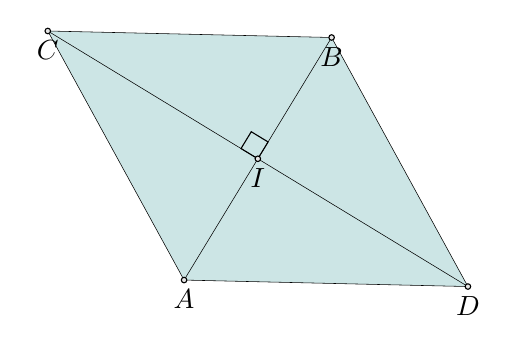
\begin{tikzpicture}[rotate=25]
  \tkzDefPoints{-2/0/A,1/2/B}
  \tkzDefLine[mediator](A,B)\tkzGetPoints{C}{D}
  \tkzDefMidPoint(A,B)\tkzGetPoint{I}

  \tkzFillPolygon[color=teal!20](A,C,B,D)
  \tkzDrawSegments(A,B C,D C,A C,B D,A D,B)
  \tkzMarkRightAngle(B,I,C)
  \tkzDrawPoints(A,B,C,D,I)
  \tkzLabelPoints(A,B,C,D,I)
\end{tikzpicture}
\end{document}
